\documentclass[UTF8,12pt,a4paper]{ctexart}

\usepackage{amsmath,amssymb,bm}
\usepackage{array,booktabs,tabularx,longtable}
\usepackage{geometry}
\usepackage{graphicx}
\usepackage{float}
\usepackage{xcolor}
\usepackage{enumitem}
\usepackage{siunitx}
\usepackage{hyperref}

\geometry{left=2.45cm,right=2.45cm,top=2.35cm,bottom=2.35cm}
\graphicspath{{../figures/}}
\hypersetup{colorlinks=true,linkcolor=blue,urlcolor=blue}
\setlength{\parindent}{2em}
\setlength{\parskip}{0.35em}
\setlength{\emergencystretch}{3em}
\renewcommand{\arraystretch}{1.18}

\title{2025 年高教社杯全国大学生数学建模竞赛 B 题\\[0.4em]
问题二：碳化硅外延层厚度的确定}
\author{独立求解与可复现数值实现}
\date{}

\begin{document}
\maketitle

\begin{abstract}
问题二要求依据问题一建立的双光束干涉模型，利用入射角为 $10^\circ$ 和
$15^\circ$ 的两组碳化硅（SiC）红外反射光谱确定同一晶圆片的外延层厚度，
并分析结果可靠性。本文先利用相邻干涉峰的波数间隔给出厚度的透明初值，
再将空气--SiC 外延层--SiC 衬底的 Fresnel 双光束模型与 Lorentz--Drude
色散模型结合，在两个入射角之间共享同一个厚度，进行全谱联合反演。为避免
把仪器的幅值归一化误差误认为厚度变化，对每个入射角引入有界线性幅值校准，
并在每次目标函数计算中解析消去该校准项。最终得到
\[
\boxed{d=7.400452153\ \mu\mathrm{m}},
\]
附件 1 和附件 2 的决定系数分别为 $0.9990855$ 和 $0.9981954$。
在最终厚度附近重新优化非厚度参数得到的 1\% MSE 局部敏感性区间为
$[7.37650,7.42278]\ \mu\mathrm{m}$。多种随机种子、双角度一致性、残差分布、
材料常数扰动和高阶往返幅度诊断共同支持该结果；同时，文中明确说明了
Lorentz--Drude 常数和仪器校准项属于建模假设，而不是附件直接提供的观测量。
\end{abstract}

\section{题面约束与本次交付范围}

题面给出的事实约束与本次实现的任务边界分开如下。

\begin{description}[leftmargin=5em]
  \item[题面事实]
  附件 1、2 来自同一块 SiC 晶圆片，入射角分别为 $10^\circ$ 和 $15^\circ$；
  每个 Excel 的第 1 列是波数 $\sigma$（单位 $\mathrm{cm}^{-1}$），第 2 列是
  反射率（单位 \%）。问题二要求根据问题一的双光束模型设计算法、计算厚度并
  分析可靠性。
  \item[本次用户任务]
  只完成问题二，产出独立的 LaTeX、数值代码、配图和结果文件；问题三的
  多光束 Si 分析不作为本文件的求解对象。
  \item[本节采用的额外假设]
  题面没有给出完整的复折射率曲线，因此为实现可计算的全谱反演，采用记录在
  结果文件中的 4H-SiC Lorentz--Drude 背景常数，并把测量百分比的线性幅值/基线
  校准作为有界 nuisance 参数。所有额外假设均不冒充题面直接给出的数据。
\end{description}

\section{数据读取与审计}

代码从独立交付目录的 \verb|data/附件1.xlsx| 和 \verb|data/附件2.xlsx| 读取
第一个工作表前两列。每份原始工作簿有 7469 行数值数据，波数升序、无重复值、
无缺失值，中位采样步长约为 $0.482\ \mathrm{cm}^{-1}$。两个文件的第一个
反射率均为精确的 $0\%$，而下一采样点已回到正常光谱范围，因此将它作为
端点异常候选：只在拟合数组中删除该一行，原始 Excel 不修改。

\begin{table}[H]
  \centering
  \caption{附件 1、2 的输入审计结果}
  \label{tab:data-audit}
  \small
  \setlength{\tabcolsep}{3pt}
  \begin{tabular}{ccccccc}
    \toprule
    附件 & 材料 & 入射角 & 原始行数 & 拟合行数 & 波数范围/$\mathrm{cm}^{-1}$ & 反射率最大值/\%\\
    \midrule
    1 & SiC & $10^\circ$ & 7469 & 7468 & $399.6747$--$4000.122$ & 95.384995\\
    2 & SiC & $15^\circ$ & 7469 & 7468 & $399.6747$--$4000.122$ & 102.739355\\
    \bottomrule
  \end{tabular}
\end{table}

附件 2 的反射率最大值略高于 $100\%$，这说明给出的百分比更接近仪器输出的
归一化响应，而不是已经完成绝对响应校正的物理反射率。该现象是引入有界幅值
校准项的直接数据依据；它不影响干涉相位随波数变化的主要信息。

\section{问题一模型在问题二中的具体化}

\subsection{几何、折射角与相位}

令空气、外延层和衬底分别编号为 $0,1,2$，外延层厚度为 $d$，入射角为
$\theta_0$，层内折射角为 $\theta_1$，波数为 $\sigma=1/\lambda$。对复折射率
仍使用 Snell 定律
\begin{equation}
  n_0\sin\theta_0=n_1(\sigma)\sin\theta_1(\sigma),
  \qquad n_0\simeq 1.
  \label{eq:snell}
\end{equation}
因此
\begin{equation}
  n_1(\sigma)\cos\theta_1(\sigma)
  =\sqrt{n_1^2(\sigma)-\sin^2\theta_0}.
  \label{eq:ncos}
\end{equation}
平方根选择实部非负、且在本文传播约定下使吸收波衰减的分支。

第一束反射光在 $0$--$1$ 表面直接反射；第二束光透射进入外延层，在 $1$--$2$
界面反射一次，再从外延层返回并透射出界面。两束光在外延层内产生一次往返，
由传播路程引起的相位差为
\begin{equation}
  \Delta(\sigma,\theta_0,d)
  =4\pi\sigma d\,n_1(\sigma)\cos\theta_1(\sigma).
  \label{eq:delta}
\end{equation}
式中若 $\sigma$ 以 $\mathrm{cm}^{-1}$ 输入，则 $d$ 必须先换算为 cm；
代码中 $d_{\mathrm{cm}}=10^{-4}d_{\mu\mathrm{m}}$。

\subsection{Fresnel 系数与双光束反射率}

对偏振 $q\in\{s,p\}$，界面 $i\to j$ 的振幅反射、透射系数分别采用
\begin{align}
 r_{ij}^{s}&=\frac{n_i\cos\theta_i-n_j\cos\theta_j}
 {n_i\cos\theta_i+n_j\cos\theta_j},
 &t_{ij}^{s}&=\frac{2n_i\cos\theta_i}
 {n_i\cos\theta_i+n_j\cos\theta_j},\\
 r_{ij}^{p}&=\frac{n_j\cos\theta_i-n_i\cos\theta_j}
 {n_j\cos\theta_i+n_i\cos\theta_j},
 &t_{ij}^{p}&=\frac{2n_i\cos\theta_i}
 {n_j\cos\theta_i+n_i\cos\theta_j}.
 \label{eq:fresnel}
\end{align}

只保留问题一规定的两束反射光时，偏振 $q$ 的复振幅为
\begin{equation}
 A_q(\sigma,\theta_0;\boldsymbol p)
 =r_{01,q}+t_{01,q}\,r_{12,q}\,t_{10,q}\exp\!\left(i\Delta\right).
 \label{eq:amplitude}
\end{equation}
附件没有给出偏振态，故将非偏振光建模为 s、p 强度的算术平均：
\begin{equation}
 R_{2b}(\sigma,\theta_0;\boldsymbol p)
 =\frac{|A_s|^2+|A_p|^2}{2}.
 \label{eq:reflectance}
\end{equation}
这一步把厚度对光谱的影响分成两个部分：Fresnel 系数控制条纹包络和基线，
式 \eqref{eq:delta} 控制条纹相位。厚度主要由相位信息识别，不能只靠某一个
峰值高度确定。

\section{SiC 色散模型与待估参数}

题面指出折射率随波长、载流子浓度变化。为把这一点纳入问题二，分别对外延层
和衬底采用复介电函数
\begin{equation}
 \varepsilon_j(\sigma)=\varepsilon_\infty
 \frac{\omega_L^2-\sigma^2-i\gamma_L\sigma}
 {\omega_T^2-\sigma^2-i\gamma_T\sigma}
 -\frac{\omega_{p,j}^2}
 {\sigma^2+i\gamma_{p,j}\sigma},
 \qquad j\in\{1,2\},
 \label{eq:ld}
\end{equation}
\begin{equation}
 n_j(\sigma)=\sqrt{\varepsilon_j(\sigma)}.
 \label{eq:index}
\end{equation}
其中第一项描述晶格振动色散，第二项为自由载流子 Drude 修正。频率量全部
使用波数单位 $\mathrm{cm}^{-1}$，因为在式 \eqref{eq:delta} 中只出现无量纲的
乘积 $\sigma d$，不需要额外引入 Hz 与角频率的换算因子。

本文固定的背景常数为
\begin{equation}
  \varepsilon_\infty=6.56,
  \qquad \omega_L=970\ \mathrm{cm}^{-1},
  \qquad \omega_T=798\ \mathrm{cm}^{-1}.
  \label{eq:constants}
\end{equation}
它们是为完成反演所采用的材料模型假设，代码和 JSON 结果中均有记录，并在
第 \ref{sec:reliability} 节做扰动检查。

将七个物理参数写成
\begin{equation}
 \boldsymbol p=
 (d,\gamma_L,\gamma_T,\omega_{p,1},\gamma_{p,1},
 \omega_{p,2},\gamma_{p,2}).
 \label{eq:parameters}
\end{equation}
两组入射角数据共享式 \eqref{eq:parameters} 的全部七个参数；其中下标 $1,2$
区分外延层与衬底，而不是区分两个入射角。这样做利用了“同一块晶圆片”的
题面信息，并避免分别拟合两个厚度。

\section{厚度初值：由问题一的峰间距公式出发}

当局部折射率近似为 $n_0$ 时，相邻同类型干涉峰的波数间隔满足
\begin{equation}
 \Delta\sigma\simeq
 \frac{1}{2d\sqrt{n_0^2-\sin^2\theta_0}},
 \qquad
 d\simeq
 \frac{1}{2\Delta\sigma\sqrt{n_0^2-\sin^2\theta_0}}.
 \label{eq:period}
\end{equation}
为减少端点和强色散区对初值的影响，代码在 $1300$--$3500\ \mathrm{cm}^{-1}$
内对反射率做 101 点、三阶 Savitzky--Golay 平滑，只把平滑结果用于找峰；
最终全谱拟合仍使用全部 7468 个未平滑数据点。取初始折射率 $n_0=2.55$，
将式 \eqref{eq:period} 中的厚度换算为 $\mu\mathrm{m}$，得到表
\ref{tab:period-init}。

\begin{table}[H]
  \centering
  \caption{相邻峰间距给出的透明厚度初值}
  \label{tab:period-init}
  \small
  \setlength{\tabcolsep}{3pt}
  \begin{tabularx}{\textwidth}{c c c X c c}
    \toprule
    附件 & 角度 & 检测峰数 & 检测到的峰波数/$\mathrm{cm}^{-1}$ &
    中位间距/$\mathrm{cm}^{-1}$ & $d_0/\mu\mathrm{m}$\\
    \midrule
    1 & $10^\circ$ & 9 &
    \begin{tabular}[t]{@{}l@{}}
    \scriptsize 1394.281, 1597.252, 1838.793, 2079.851, 2323.320,\\
    \scriptsize 2582.217, 2838.221, 3094.225, 3346.854
    \end{tabular} &
    248.049 & 7.923219\\
    2 & $15^\circ$ & 9 &
    \begin{tabular}[t]{@{}l@{}}
    \scriptsize 1406.816, 1605.931, 1859.042, 2099.136, 2391.299,\\
    \scriptsize 2611.144, 2869.559, 3127.491, 3382.049
    \end{tabular} &
    253.8345 & 7.764755\\
    \bottomrule
  \end{tabularx}
\end{table}

两个角度的粗略厚度相差约 $2.00\%$，主要是由于折射率色散、峰定位误差和
条纹包络变化；因此这里的 $d_0$ 只作为搜索起点和尺度检查，不能直接作为最终
答案。图 \ref{fig:init} 给出平滑光谱与检测峰，说明峰间距随波数并非严格常数。

\begin{figure}[H]
  \centering
  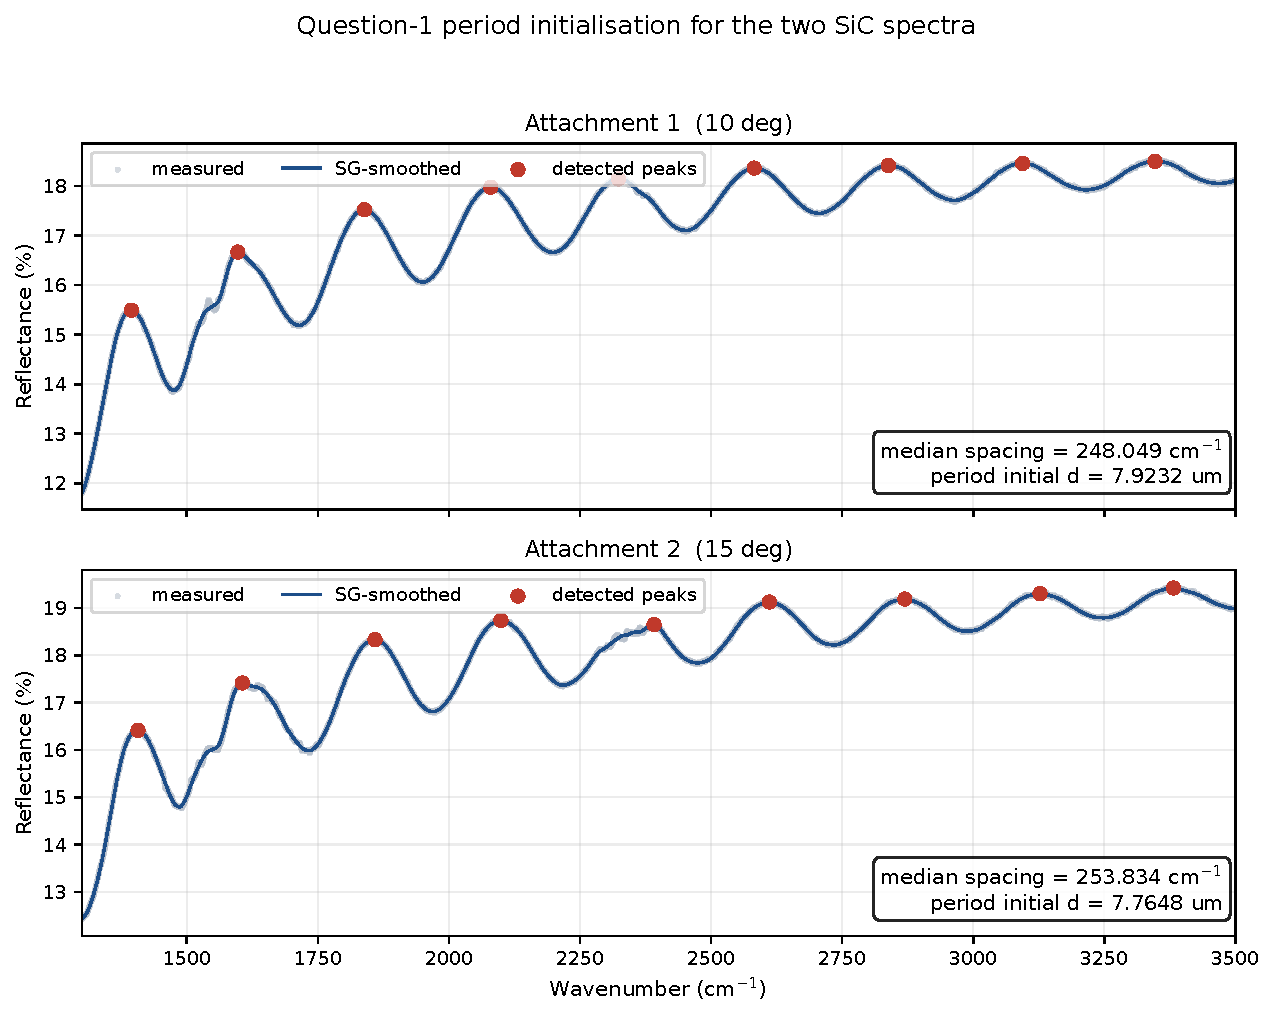
\includegraphics[width=0.98\textwidth]{fig_q2_initial_peaks.pdf}
  \caption{附件 1、2 的平滑光谱和用于厚度初值的峰检测}
  \label{fig:init}
\end{figure}

\section{双角度联合反演算法}

\subsection{测量幅值校准与目标函数}

令 $\widetilde y_{ji}=100R_{2b}(\sigma_{ji},\theta_j;\boldsymbol p)$ 为
Fresnel 模型给出的百分比反射率，$y_{ji}$ 为附件中的观测百分比。考虑仪器
归一化、基线和不同角度的响应差异，使用
\begin{equation}
 y_{ji}\simeq a_j\widetilde y_{ji}+b_j,
 \qquad 0.25\leq a_j\leq1.75,
 \quad -30\leq b_j\leq30.
 \label{eq:calibration}
\end{equation}
这里 $a_j,b_j$ 是测量校准项，不是材料参数。对固定的 $\boldsymbol p$，令
$\boldsymbol X_j=[\widetilde{\boldsymbol y}_j,\boldsymbol 1]$，则无界最小二乘解为
\begin{equation}
 \begin{bmatrix}a_j\\b_j\end{bmatrix}_{\!\mathrm{LS}}
 = (\boldsymbol X_j^{\mathsf T}\boldsymbol X_j)^{-1}
 \boldsymbol X_j^{\mathsf T}\boldsymbol y_j.
 \label{eq:variable-projection}
\end{equation}
代码先把 $a_j$ 投影到其有界区间，再用固定后的 $a_j$ 重新计算最优 $b_j$ 并投影到基线边界。这样每次评价物理参数时，校准项都被解析消去，不需要让差分进化额外搜索四个近似线性参数；这种做法称为变量投影，实质是“给定非线性参数后先把线性参数解到最好”。

将两组附件等权合并，目标函数为
\begin{equation}
 J(\boldsymbol p)=
 \frac{1}{N_1+N_2}
 \sum_{j=1}^{2}\sum_{i=1}^{N_j}
 \left[a_j\widetilde y_{ji}(\boldsymbol p)+b_j-y_{ji}\right]^2.
 \label{eq:objective}
\end{equation}
由于 $N_1=N_2=7468$，式 \eqref{eq:objective} 等价于两个入射角 MSE 的算术平均。
拟合指标定义为
\begin{align}
 \mathrm{RMSE}_j&=\sqrt{\frac{1}{N_j}\sum_i e_{ji}^2},\\
 R_j^2&=1-\frac{\sum_i e_{ji}^2}
 {\sum_i(y_{ji}-\bar y_j)^2},
 \qquad e_{ji}=\widehat y_{ji}-y_{ji}.
 \label{eq:metrics}
\end{align}
RMSE 的单位仍是反射率百分点，$R^2$ 衡量模型解释观测波动的比例。

\subsection{参数边界与优化步骤}

使用如下宽边界保证阻尼为正，同时将厚度限制在峰间距初值附近的同一相位分支：
\begin{table}[H]
  \centering
  \caption{七个物理参数的搜索边界}
  \label{tab:bounds}
  \small
  \begin{tabular}{ccc}
    \toprule
    参数 & 搜索范围 & 物理含义\\
    \midrule
    $d/\mu\mathrm{m}$ & $[3,12]$ & 外延层厚度\\
    $\gamma_L,\gamma_T/\mathrm{cm}^{-1}$ & $[0.1,1500]$ & 晶格阻尼\\
    $\omega_{p,1},\omega_{p,2}/\mathrm{cm}^{-1}$ & $[1,5000]$ & 层/衬底等离子体频率\\
    $\gamma_{p,1},\gamma_{p,2}/\mathrm{cm}^{-1}$ & $[0.1,2000]$ & 层/衬底载流子阻尼\\
    \bottomrule
  \end{tabular}
\end{table}

差分进化（DE）适合处理含有周期相位、强色散和多个局部极小值的非线性目标。
它维护一群候选参数，用候选向量之间的差分进行变异，再通过交叉和目标函数
选择保留更优个体；它不需要目标函数可导。本文先把各参数线性归一化到 $[0,1]$，
在每隔 12 个点抽取一个数据点的子样本上以种子 2025、2718、3141 分别运行 DE，
然后把每个种子的局部最优解交给 L-BFGS-B。L-BFGS-B 是带边界的梯度型局部
优化器，适合在已接近最优点后利用完整数据做精修。最后再用 7468+7468 个
数据点重新计算预测和所有指标。

\begin{enumerate}[label=步骤\arabic*：,leftmargin=5em]
  \item 读取两份工作簿，检查波数单调性、缺失值、重复值，并剔除首个 0\% 端点；
  \item 在 $1300$--$3500\ \mathrm{cm}^{-1}$ 波段平滑找峰，用式
  \eqref{eq:period} 得到 $d_0$；
  \item 对给定 $\boldsymbol p$ 计算式 \eqref{eq:ld}--\eqref{eq:reflectance}，
  分别求两个角度的幅值/基线校准项，再计算式 \eqref{eq:objective}；
  \item 以三个固定种子进行 DE 搜索，用 L-BFGS-B 在子样本上局部精修，选取
  子样本 MSE 最小的候选；
  \item 在完整数据上精修并输出共同厚度、两个角度的拟合指标、预测 CSV、
  厚度剖面、材料常数扰动结果和高阶往返幅度诊断。
\end{enumerate}

\begin{figure}[H]
  \centering
  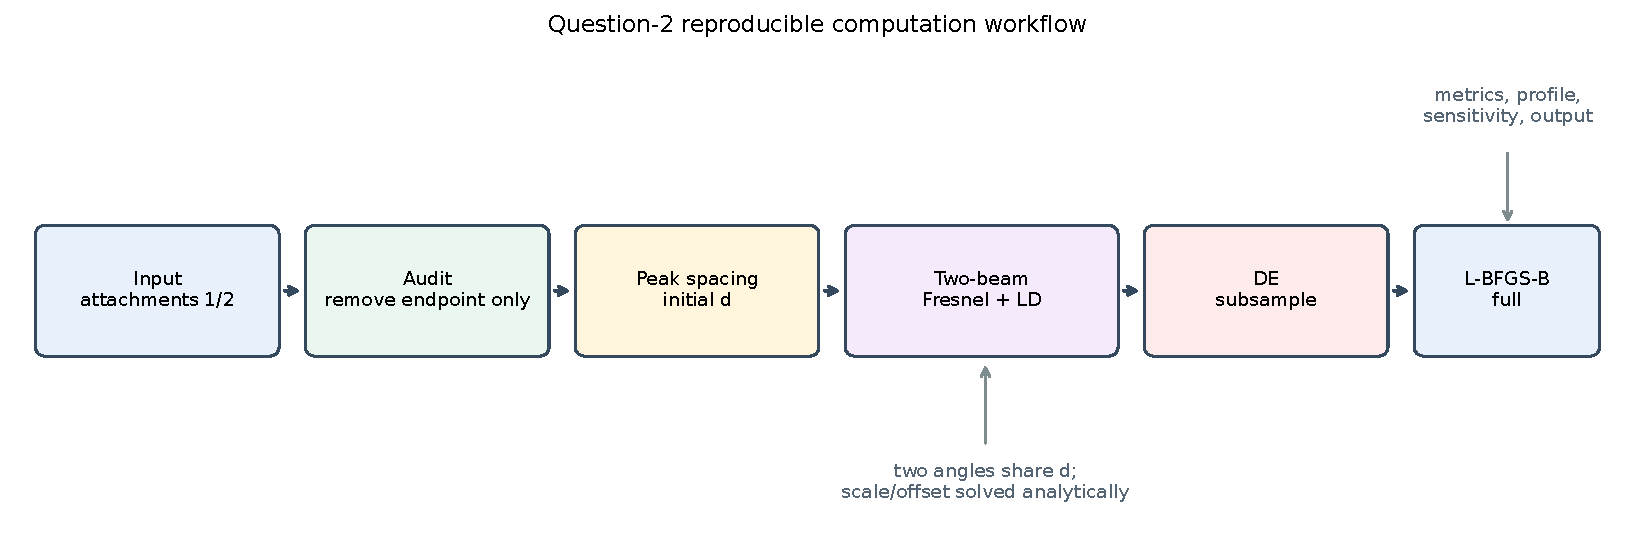
\includegraphics[width=0.98\textwidth]{fig_q2_workflow.pdf}
  \caption{问题二双角度联合反演的可复现流程}
  \label{fig:workflow}
\end{figure}

\section{数值结果}

\subsection{联合拟合参数}

完整数据精修的最优物理参数如表 \ref{tab:parameters}。参数 $\gamma_L$ 到达
搜索边界 $0.1\ \mathrm{cm}^{-1}$，说明该参数在当前数据和其他 nuisance 参数
之间存在相关性，不宜把所有参数都解释为独立、唯一的材料测量值；厚度由两个
角度共同的相位变化支持，是本文的主要报告量。

\begin{table}[H]
  \centering
  \caption{SiC 双光束联合拟合的物理参数}
  \label{tab:parameters}
  \small
  \begin{tabular}{ccc}
    \toprule
    参数 & 数值 & 单位\\
    \midrule
    $d$ & $7.400452153$ & $\mu\mathrm{m}$\\
    $\gamma_L$ & $0.100000$ & $\mathrm{cm}^{-1}$\\
    $\gamma_T$ & $2.558084$ & $\mathrm{cm}^{-1}$\\
    $\omega_{p,1}$ & $473.848563$ & $\mathrm{cm}^{-1}$\\
    $\gamma_{p,1}$ & $1184.132748$ & $\mathrm{cm}^{-1}$\\
    $\omega_{p,2}$ & $1123.258434$ & $\mathrm{cm}^{-1}$\\
    $\gamma_{p,2}$ & $611.594793$ & $\mathrm{cm}^{-1}$\\
    \bottomrule
  \end{tabular}
\end{table}

对应的线性校准项为
\begin{table}[H]
  \centering
  \caption{两个入射角的幅值与基线校准项}
  \label{tab:calibration}
  \small
  \begin{tabular}{cccc}
    \toprule
    附件 & 入射角 & $a_j$ & $b_j$/\%\\
    \midrule
    1 & $10^\circ$ & 0.9755607 & 0.0314805\\
    2 & $15^\circ$ & 1.0524134 & -0.4043959\\
    \bottomrule
  \end{tabular}
\end{table}

\subsection{拟合曲线与指标}

图 \ref{fig:fit} 中橙色曲线是同一个厚度和同一组材料参数在两个角度下的
联合拟合，灰色曲线是实测数据；下方给出逐点残差。强色散/吸收区域附近的
尖锐结构对复折射率和仪器响应最敏感，因此局部残差明显大于平坦尾段。

\begin{figure}[H]
  \centering
  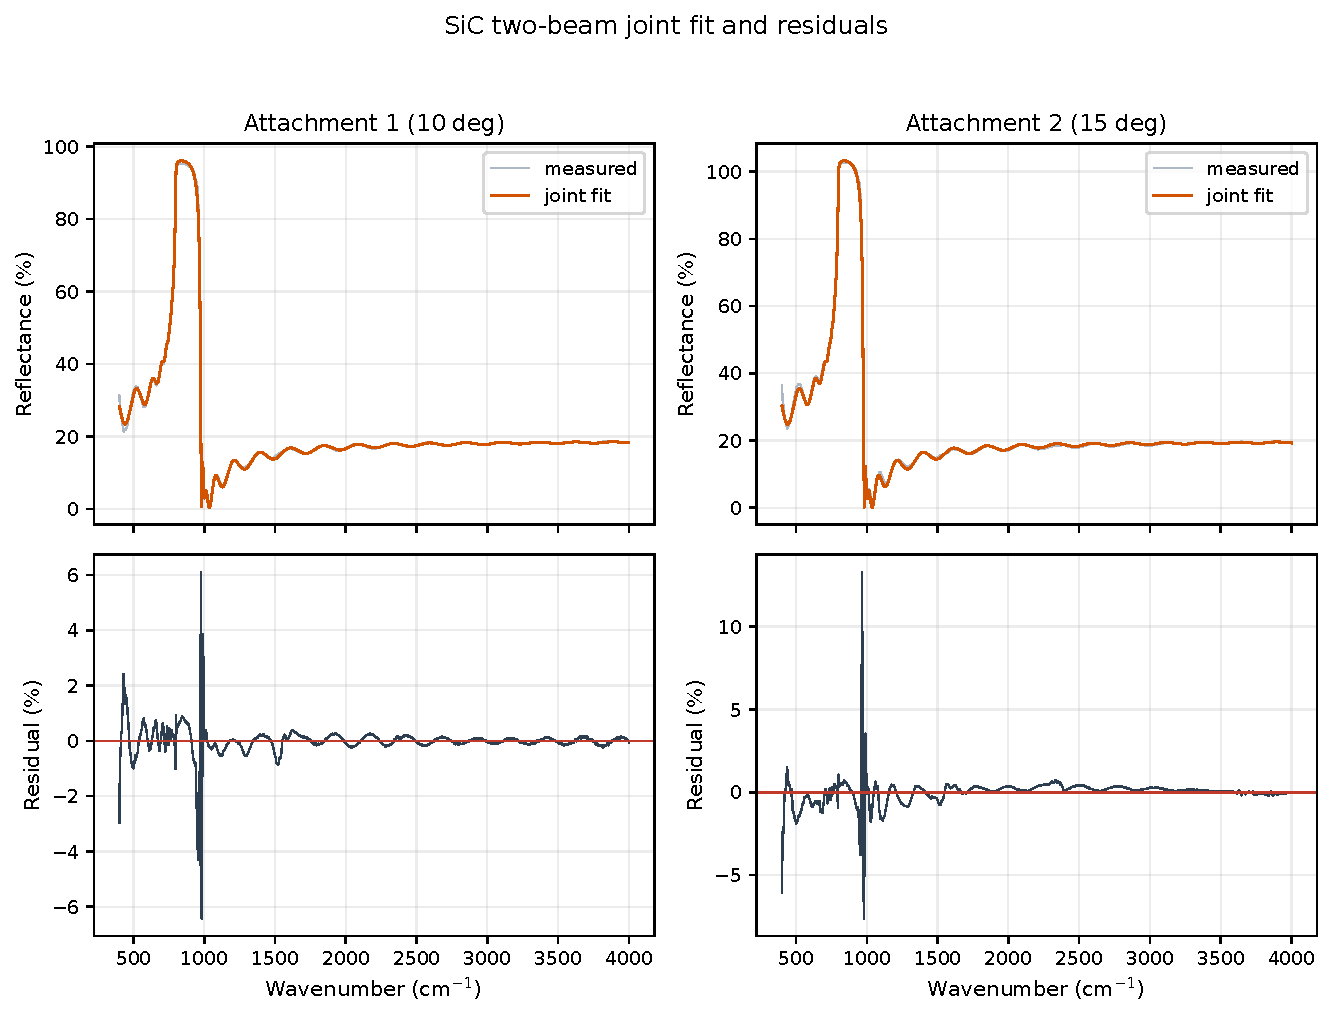
\includegraphics[width=0.99\textwidth]{fig_q2_fit_residual.pdf}
  \caption{附件 1、2 的全谱联合拟合和残差}
  \label{fig:fit}
\end{figure}

\begin{table}[H]
  \centering
  \caption{两个附件的拟合指标}
  \label{tab:metrics}
  \small
  \begin{tabular}{ccccccc}
    \toprule
    附件 & 角度 & RMSE/\% & MAE/\% & $R^2$ & $|e|$ 中位数/\% & $|e|$ 95\%分位/\%\\
    \midrule
    1 & $10^\circ$ & 0.531845 & 0.240775 & 0.9990855 & 0.120811 & 0.772624\\
    2 & $15^\circ$ & 0.806417 & 0.376479 & 0.9981954 & 0.219691 & 1.216826\\
    \bottomrule
  \end{tabular}
\end{table}

因此，按本节明确的双光束、Lorentz--Drude 和线性校准假设，问题二的厚度结果为
\begin{equation}
  \boxed{d=7.400452153\ \mu\mathrm{m}\approx 7.4005\ \mu\mathrm{m}}.
  \label{eq:final-d}
\end{equation}

\section{可靠性与敏感性分析}
\label{sec:reliability}

\subsection{数据、角度和优化稳定性}

首先，输入审计显示两份附件的波数网格一致且没有缺失、重复或非单调问题，
仅删除了两个共同位于开头的 0\% 端点；删除规则对两组数据完全一致。其次，
峰间距初值分别为 $7.923219$ 和 $7.764755\ \mu\mathrm{m}$，虽然存在约
$2\%$ 的粗估差异，但联合拟合用同一个 $d$ 同时解释两个入射角，并取得表
\ref{tab:metrics} 中的高 $R^2$，说明相位尺度跨角度保持一致。

三组 DE 种子在子样本局部精修后的结果如下。表中的 $d$ 是子样本局部候选，
不是把每个候选都重新进行完整数据精修后的独立置信区间；它用于检验优化是否
被某一个随机种子控制。

\begin{table}[H]
  \centering
  \caption{不同 DE 种子的子样本局部结果}
  \label{tab:seeds}
  \small
  \begin{tabular}{cccc}
    \toprule
    种子 & DE 子样本 MSE & 局部精修 MSE & 局部厚度/$\mu\mathrm{m}$\\
    \midrule
    2025 & 0.492784950 & 0.476948040 & 7.397358789\\
    2718 & 0.479191845 & 0.476948040 & 7.397358920\\
    3141 & 0.482476274 & 0.476948040 & 7.397358823\\
    \bottomrule
  \end{tabular}
\end{table}

三个局部厚度的极差约为 $1.3\times10^{-7}\ \mu\mathrm{m}$，而完整数据精修后
目标函数为 $J=0.466583777\ (\% )^2$。这说明在给定边界和模型下，优化结果
具有很好的重复性；但差分进化是高质量的数值搜索，并不构成数学意义上的全局
最优性证明。

\subsection{厚度剖面敏感性}

为了避免只看优化器终点，固定厚度 $d$，对其余六个物理参数重新做 L-BFGS-B
局部优化，并记录重新优化后的 $J(d)$。以相对最优 MSE 增加 $1\%$ 作为一个
局部辨识尺度，线性插值得到
\begin{equation}
  d\in[7.376503934,\ 7.422775503]\ \mu\mathrm{m}.
  \label{eq:profile-interval}
\end{equation}
该区间半宽 $0.0231358\ \mu\mathrm{m}$，相对半宽约 $0.3126\%$；它是
“重新优化 nuisance 参数后的局部敏感性区间”，不是由独立重复测量或概率噪声
模型推导出的正式置信区间。图 \ref{fig:profile} 显示了该剖面在最优厚度附近
具有清晰单谷结构。

\begin{figure}[H]
  \centering
  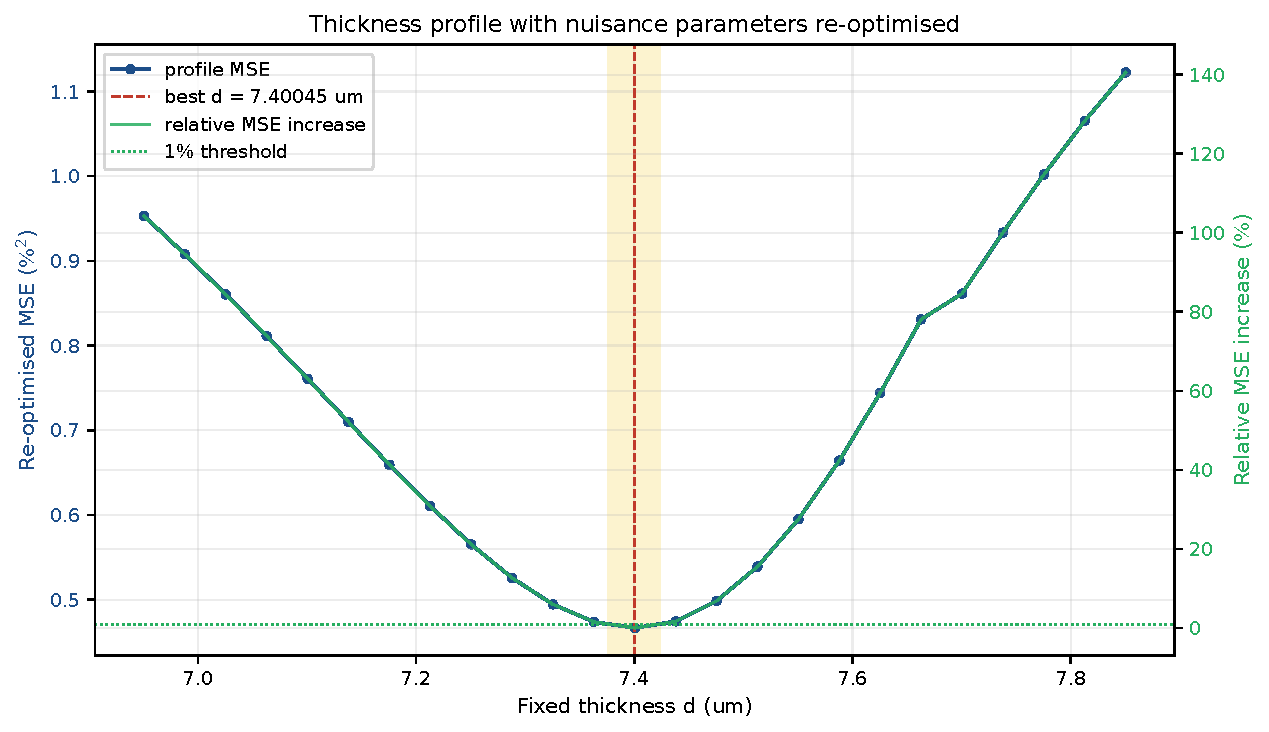
\includegraphics[width=0.98\textwidth]{fig_q2_thickness_profile.pdf}
  \caption{固定厚度并重新优化其余参数得到的 MSE 剖面}
  \label{fig:profile}
\end{figure}

\subsection{材料背景常数的局部扰动}

将 $\varepsilon_\infty,\omega_L,\omega_T$ 分别固定扰动 $\pm2\%$，其余六个
物理参数固定在基准解，只在基准厚度 $\pm0.45\ \mu\mathrm{m}$ 的局部相位分支
内重新优化厚度。结果为
\begin{table}[H]
  \centering
  \caption{材料常数 $\pm2\%$ 局部条件敏感性}
  \label{tab:material-sensitivity}
  \small
  \begin{tabular}{ccccc}
    \toprule
    扰动参数 & 扰动 & 条件厚度/$\mu\mathrm{m}$ & 相对厚度变化 & 条件 MSE/$({\%})^2$\\
    \midrule
    $\varepsilon_\infty$ & $-2\%$ & 7.478912 & +1.0602\% & 0.465596\\
    $\varepsilon_\infty$ & $+2\%$ & 7.324361 & -1.0282\% & 0.479618\\
    $\omega_L$ & $-2\%$ & 7.360531 & -0.5394\% & 26.700960\\
    $\omega_L$ & $+2\%$ & 7.444629 & +0.5969\% & 21.664478\\
    $\omega_T$ & $-2\%$ & 7.361689 & -0.5238\% & 4.566652\\
    $\omega_T$ & $+2\%$ & 7.429958 & +0.3987\% & 5.297012\\
    \bottomrule
  \end{tabular}
\end{table}

该表有两个重要含义：第一，若材料背景常数只发生小幅变化，厚度在局部相位
分支内的变化约为 $0.4$--$1.1\%$；第二，某些常数的扰动会令光谱形状误差
显著上升，即“拟合损失”比“厚度变化”更敏感。不能把表中的条件厚度范围直接
当作统计误差，也不能把到边界的阻尼参数解释成唯一材料常数。

\begin{figure}[H]
  \centering
  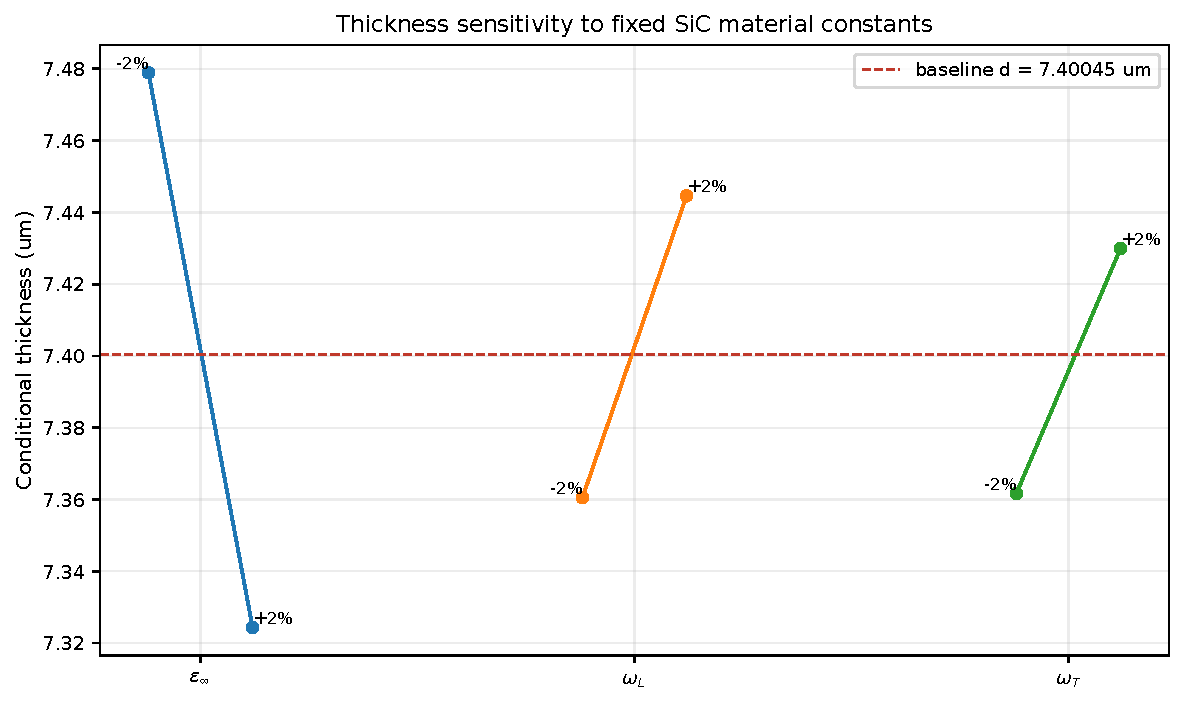
\includegraphics[width=0.90\textwidth]{fig_q2_material_sensitivity.pdf}
  \caption{SiC 背景材料常数局部扰动下的条件厚度}
  \label{fig:sensitivity}
\end{figure}

\subsection{双光束截断的高阶往返诊断}

虽然问题二按题意采用双光束模型，但可以用拟合后的 Fresnel 系数检查被省略的
下一次内部往返是否可能很大。一次额外往返对振幅的乘子近似为
\begin{equation}
 \rho_q(\sigma)=\left|r_{10,q}r_{12,q}\exp(i\Delta)\right|.
 \label{eq:rho}
\end{equation}
代码对 s、p 两偏振取平均后得到：附件 1 的 $\rho$ 中位数、95\%分位和最大值
分别为 $0.002995,0.022511,0.066781$；附件 2 分别为
$0.002993,0.022414,0.060790$。大多数波数处额外往返振幅只有千分之几，
说明在当前数据精度下双光束厚度对高阶返回不敏感；但该量是基于模型参数的
诊断，不等同于直接测得仪器相干长度或界面粗糙度。

\section{结论、适用范围与复现方式}

\subsection{结论}

在附件 1、2 的数据口径下，本文用问题一的双光束 Fresnel 模型建立了一个
共享厚度的全谱联合反演算法。峰间距法给出 $7.923219$ 和 $7.764755\ \mu$m
的初步尺度；在考虑 SiC 色散、s/p 偏振平均和测量幅值校准后，完整联合反演的
主要结果为
\[
\boxed{d=7.400452153\ \mu\mathrm{m}\quad (\text{建议报告 }7.4005\ \mu\mathrm{m})}.
\]
两个入射角的 $R^2$ 分别为 $0.9990855$ 和 $0.9981954$，局部 1\% MSE 敏感性
区间为 $[7.37650,7.42278]\ \mu$m。多种子重复、双角度共享厚度和高阶往返
幅度诊断均支持该厚度在当前模型和测量精度下的稳定性。

\subsection{局限性}

\begin{enumerate}[leftmargin=5em]
  \item 题面没有提供完整复折射率或仪器响应曲线，式 \eqref{eq:constants} 的
  材料背景常数是可复现的外部建模假设；若有实测光学常数，应优先替换并重新运行。
  \item 幅值校准项改善了对百分比响应的拟合，但增加了模型自由度；若仪器已经
  完成绝对反射率校准，可以固定 $a_j=1,b_j=0$ 并重新比较厚度。
  \item $\gamma_L$ 到达边界，表明 nuisance 参数存在相关性。本文只把厚度作为
  主结果，不把其余参数包装成独立材料测量结论。
  \item 1\% MSE 区间是局部数值敏感性指标，不是严格概率置信区间；正式不确定度
  还需要测量重复、噪声分布、偏振态和仪器响应函数。
\end{enumerate}

\subsection{可复现文件与命令}

本交付目录为
\verb|F:/数学建模/2025B/题目2_完整交付|，其中：
\begin{itemize}[leftmargin=5em]
  \item \verb|code/solve_q2.py|：读取附件、建立前向模型、优化并输出数值结果；
  \item \verb|code/make_q2_figures.py|：只读取结果文件并生成本文五类 PDF/PNG 图；
  \item \verb|results/q2_fit.json|：参数、指标、种子记录、敏感性和输入审计汇总；
  \item \verb|results/q2_predictions.csv|：两个附件的逐点模型预测和残差；
  \item \verb|results/q2_thickness_profile.csv|：固定厚度剖面；
  \item \verb|figures/|：本文引用的矢量 PDF 和预览 PNG。
\end{itemize}

在交付目录根部运行：
\begin{verbatim}
C:\Python313\python.exe code\solve_q2.py
C:\Python313\python.exe code\make_q2_figures.py
\end{verbatim}
然后在 \verb|paper| 目录连续编译两遍：
\begin{verbatim}
xelatex -interaction=nonstopmode -halt-on-error -file-line-error \
  -output-directory=build q2_solution.tex
xelatex -interaction=nonstopmode -halt-on-error -file-line-error \
  -output-directory=build q2_solution.tex
\end{verbatim}
输出 PDF 为 \verb|paper/build/q2_solution.pdf|。实际运行的 Python、NumPy 和平台
信息已写入 \verb|results/q2_fit.json|，输入附件 SHA-256 也写入
\verb|results/data_audit.json|。

\end{document}
